\chapter{Realisierung}\label{AppendixRealisierung}

\section{HTML-Prototyp}

Der HTML-Prototyp ist im Verzeichnis «html-prototype» zu finden, dieser wurde
mit \textbf{Ember.js} und \textbf{SASS} umgesetzt.
Um den Prototypen zu starten muss \textbf{Node.js} und \textbf{Yarn} installiert sein.


\noindent
Den Prototypen kann man mit dem folgenden Kommando starten:

\begin{lstlisting}[language=bash,frame=single]
$ yarn && yarn start
\end{lstlisting}

\noindent
Danach kann der Prototyp über die URL \url{http://localhost:4200/} geöffnet werden.

\noindent
Folgende URLs sind verfügbar:

\begin{itemize}
  \tightlist{}
  \item{} \url{http://localhost:4200/}
  \item{} \url{http://localhost:4200/search}
  \item{} \url{http://localhost:4200/gig-detail}
  \item{} \url{http://localhost:4200/add-gig}
  \item{} \url{http://localhost:4200/login}
  \item{} \url{http://localhost:4200/register}
\end{itemize}

\clearpage
\section{Projekt Setup}

Die Initialisierung des Projekts wurde mit der Phoenix Framework «Umbrella»
Struktur erstellt.

\begin{lstlisting}[language=bash,frame=single]
$ mix phx.new gigpillar --umbrella
\end{lstlisting}

Die Umbrella Struktur trennt die Applikation in kleinere Teilapplikationen,
dies ermöglicht eine klarere Trennung zwischen der Webapplikation und der Businesslogik.

\noindent
Erläuterung der Projekt/Dateistruktur:

\begin{lstlisting}[frame=single]
/apps/gigpillar/
\end{lstlisting}
Die Gigpillar Grundapplikation

\begin{lstlisting}[frame=single]
# Die Gigpillar Webapplikation
/apps/gigpillar_web/
# Applikations{\"u}bergreifende Konfigurationsfiles
/config/
# Die Projektdokumentation
/doc/
# Der HTML-Prototyp
/html-prototype/
# Die Dockerkonfiguration f{\"u}r die Entwicklungsumgebung
/docker-compose.yml
# Die applikationsubergreiffenden Abhangigkeiten
/mix.exs
\end{lstlisting}

\section{Dependency Management}

Für das Dependency Management, wurde ein Bot eingerichtet, der
Benachrichtigungen, bzw. Pull-Requests, bei Updates zustellt.

Für das Projekt wurde der Bot «Dependabot»\footnote{\url{https://github.com/marketplace/dependabot}} ausgewählt, da diser Elixir sowie JavaScript Abhängigkeiten unterstützt.

Durch die Benützung des Dependabot, können während der Entwicklung des Projektes
die Software Abhängigkeiten jederzeit auf dem neusten Stand gehalten werden.

\clearpage
\subsection{Datenbankschema}

\subsubsection{Alle Entitäten}
Alle «created\_at» Felder wurden nach «inserted\_at» umbenannt, da dies die
Standardbenennung des Phoenix Frameworks ist.

\subsubsection{User}
Der Benutzer Entität wurde das Feld «password» nach «password\_hash» umbenannt,
damit klar ist, dass nicht ein Passwort sondern nur ein Hash abgespeichert wird.

\subsubsection{Genre}
Der Genre Entität sind im Konzept die Datumsfelder «update\_at» und «inserted\_at»
vergessen gegangen und wurden in der Realisierung nachgeführt.

\subsubsection{Gig}
In der Gig Entität wurden drei weitere Felder hinzugefügt.
Die Felder «uuid» und «picture» dienen dazu, die beim Erfassen sowie
Bearbeiten eines Gigs hochgeladenen Bilder zu identifizieren.
Das zusätzliche Feld «tickets» ermöglicht es, beim Erfassen eines Gigs
einen Link zum Ticketvorverkauf zu hinterlegen.

\subsubsection{Location}
Die Location Entität erhielt bei der Realisierung zwei neue Felder,
«address» für die Adresse der Location und
«google\_place\_id» um die Referenz der Google API zu erhalten.

\clearpage
\subsubsection{Finales Schema}

\begin{figure}[!htb]
  \centering
  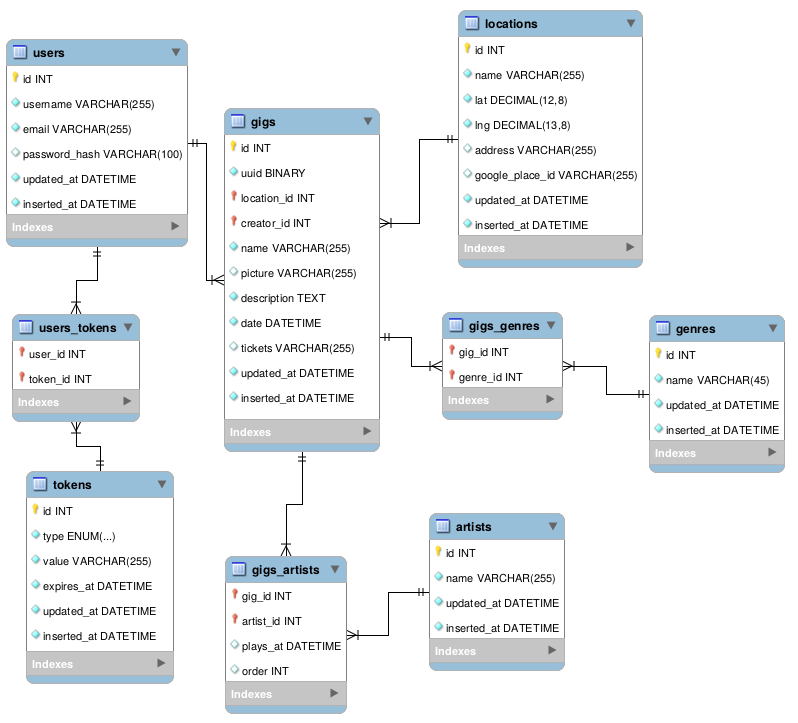
\includegraphics[width=0.95\textwidth]{realisierung/erd.png}
  \caption{Realisierung: Entity Relationship Diagram}
\end{figure}

\clearpage
\subsection{Berechtigungssystem}

Das Bearbeiten von Gigs wurde so eingeschränkt, dass nur angemeldete Benutzer Gigs erstellen dürfen und Benutzer nur eigene Gigs bearbeiten können.

Dazu wurde die Library «Canary»\footnote{\url{https://github.com/cpjk/canary}} verwendet. In der Datei «apps/gigpillar/lib/abilities.ex» wurden die Berechtigungen wie gefolgt umgesetzt:

\lstinputlisting[language=elixir,frame=single]{../apps/gigpillar/lib/abilities.ex}

\clearpage
\subsection{Location Autocomplete}

Das Location Autocomplete Feld wurde mit der «Google Place API»\footnote{\url{https://developers.google.com/places/web-service/autocomplete}} umgesetzt.

Die verwendete Library «google-api-elixir-client» implementiert die
Autocomplete API, jedoch fehlte noch die entsprechende Zusatzfunktion um
weitere Details, wie die geographischen Koordinaten, Adresse, etc., zu den gefundenen Locations abzufragen.

Die API um Details abzufragen wurden im Rahmen von diesem Projekt umgesetzt
und zurück an das originale Projekt beigesteuert.

Ausserdem musste eine Abhängigkeit auf den aktuellsten Stand gebracht werden.

Die beiden Beiträge für die Library sind auf Github zu finden:

\begin{itemize}
  \item{} \url{https://github.com/seanabrahams/google-api-elixir-client/pull/10/files}
  \item{} \url{https://github.com/seanabrahams/google-api-elixir-client/pull/11/files}
\end{itemize}

\clearpage
\subsection{HTML Erweiterungen}

\subsubsection{<search-box>}

\subsubsection{<with-dropdown>}

\subsubsection{<location-input>}

\subsubsection{<picture-input>}

\subsubsection{<datetime-input>}

\subsubsection{<artists-input>}

\clearpage
\subsection{Asset Optimierungen}

- html minifier
- imagemin
- terser
- external helpers

\clearpage
\subsection{File Upload}

- minio
- resizing
- uuid
- asset host config

\subsection{Openstreetmap}

- calc

\clearpage
\section{Probleme}

\clearpage
\section{Offene Punkte}

\clearpage
\section{Tests}

\section{Auswertung}
